% Standalone Helix: 28 Oct 2026 Research Meeting
% Visual style follows the 21 Oct 2026 light Madrid decks.
% Facts are taken from the local ASPLOS '25 PDF only.
% Compile with pdfLaTeX from this directory. Keep Helix/ beside this file.
\documentclass[aspectratio=169,10pt]{beamer}
\usepackage[english]{babel}
\usepackage[utf8]{inputenc}
\usepackage[T1]{fontenc}
\usepackage{lmodern}
\usepackage{amsmath,amssymb}
\usepackage{booktabs,tabularx,array}
\usepackage{graphicx}
\graphicspath{{./}{figures/}}
\usepackage{xcolor}
\usepackage{tikz}
\usetikzlibrary{arrows.meta,positioning,calc,shapes.geometric}
\usepackage{hyperref}

\usetheme{Madrid}
\usecolortheme{default}
\definecolor{Ink}{HTML}{243748}
\definecolor{Muted}{HTML}{667B8B}
\definecolor{Accent}{HTML}{347E74}
\definecolor{AccentBlue}{HTML}{507DAD}
\definecolor{SoftMint}{HTML}{E6F4EE}
\definecolor{SoftBlue}{HTML}{E9F2F9}
\definecolor{SoftLilac}{HTML}{F1EEF8}
\definecolor{Paper}{HTML}{FBFCFE}
\definecolor{Divider}{HTML}{D8E4EB}

\setbeamercolor{background canvas}{bg=Paper}
\setbeamercolor{normal text}{fg=Ink}
\setbeamercolor{structure}{fg=Accent}
\setbeamercolor{frametitle}{fg=Ink,bg=SoftBlue}
\setbeamercolor{title}{fg=Ink}
\setbeamercolor{subtitle}{fg=Muted}
\setbeamercolor{block title}{fg=Ink,bg=SoftBlue}
\setbeamercolor{block body}{fg=Ink,bg=white}
\setbeamercolor{item}{fg=Accent}
\setbeamercolor{caption name}{fg=Muted}
\setbeamercolor{footline}{fg=Muted,bg=Paper}
\setbeamerfont{frametitle}{size=\large,series=\bfseries}
\setbeamerfont{footline}{size=\tiny}
\setbeamerfont{block title}{series=\bfseries}
\setbeamertemplate{headline}{}
\setbeamertemplate{navigation symbols}{}
\setbeamertemplate{blocks}[rounded][shadow=false]
\setbeamertemplate{itemize items}[circle]
\setbeamertemplate{itemize subitem}[circle]
\setbeamertemplate{footline}{%
  \leavevmode\hbox{%
    \begin{beamercolorbox}[wd=\paperwidth,ht=.30cm,dp=.16cm,rightskip=.60cm plus 1fil]{footline}%
      \hfill\insertframenumber\,/\,\inserttotalframenumber
    \end{beamercolorbox}}}
\setbeamertemplate{frametitle}{%
  \nointerlineskip
  \begin{beamercolorbox}[wd=\paperwidth,ht=.72cm,dp=.16cm,leftskip=.55cm,rightskip=.40cm]{frametitle}%
    \usebeamerfont{frametitle}\insertframetitle
  \end{beamercolorbox}}

\newcommand{\smalllabel}[1]{{\scriptsize\bfseries\color{Accent}\MakeUppercase{#1}}}
\newcommand{\hint}[1]{{\footnotesize\color{Muted}#1}}
\newcommand{\takeaway}[1]{%
  \begin{beamercolorbox}[rounded=true,sep=0.15cm,wd=\linewidth]{block title}%
    {\small\bfseries #1}
  \end{beamercolorbox}}
\newcommand{\stepcard}[3]{%
  \begin{beamercolorbox}[rounded=true,sep=0.16cm,wd=\linewidth]{block body}%
    {\footnotesize\bfseries\color{Accent}#1}\par\vspace{.8mm}
    {\normalsize\bfseries #2}\par\vspace{.8mm}
    {\footnotesize\color{Muted}#3}%
  \end{beamercolorbox}}

\newcommand{\figureplaceholder}[3]{%
  \begingroup\centering
  \IfFileExists{#1}{%
    \includegraphics[width=.98\linewidth,height=#2,keepaspectratio]{#1}%
  }{%
    \IfFileExists{figures/#1}{%
      \includegraphics[width=.98\linewidth,height=#2,keepaspectratio]{figures/#1}%
    }{%
      \begin{tikzpicture}
        \node[draw=AccentBlue!55,dashed,line width=.7pt,rounded corners=4pt,
              fill=SoftBlue!60,minimum height=#2,minimum width=.95\linewidth,
              text width=.85\linewidth,align=center,inner sep=2mm] {
           {\color{AccentBlue}\bfseries FIGURE PLACEHOLDER}\\[2.2mm]
           {\color{Ink}\small #3}\\[1.5mm]
           {\color{Muted}\scriptsize\ttfamily\detokenize{#1}}};
      \end{tikzpicture}%
    }%
  }\par\endgroup}

\newcommand{\src}[1]{\vspace{0.12cm}\hint{Source: #1}}


\newcommand{\mainfig}[2]{%
  \begingroup\centering
  \includegraphics[width=\linewidth,height=#2,keepaspectratio]{#1}\par
  \endgroup}
\newif\ifbackup
\setbeamertemplate{footline}{\leavevmode\hbox{\begin{beamercolorbox}[wd=\paperwidth,ht=.30cm,dp=.16cm,rightskip=.60cm]{footline}\hfill\ifbackup Backup\quad PDF \insertframenumber\else Main \insertframenumber/13\fi\end{beamercolorbox}}}
\title{Heterogeneous Model Serving at Different Granularities: Helix and Tessera}
\author{Yu-Jui Liang}
\date{28 Oct 2026}
\subject{Research meeting, 28 Oct 2026}
\begin{document}
\begin{frame}[plain]

\vspace{.48cm}
\smalllabel{Research meeting}\par\vspace{.32cm}
{\LARGE\bfseries Heterogeneous Model Serving\\[.14cm]at Different Granularities:\\[.14cm]Helix and Tessera\par}
\vspace{.32cm}{\large\color{Muted}Helix (ASPLOS 2025) + Tessera\par}
\vspace{.26cm}{\Large\textbf{Yu-Jui Liang}\par}
\vspace{.10cm}{\large Advisor: Hsiang-Yun Cheng\par}
\vspace{.08cm}{\large National Taiwan University \quad | \quad Academia Sinica\par}
\vspace{.08cm}{\large 28 Oct 2026\par}
\vfill
{\footnotesize\color{Muted}Helix: Yixuan Mei et al., ASPLOS 2025\\
Tessera: Tiancheng Hu et al., arXiv:2604.10180v2}\par
\vspace{.08cm}{\color{Accent}\rule{\textwidth}{.7pt}}

\end{frame}

\begin{frame}[t]{Put the Two Papers on One Map}

\small
\renewcommand{\arraystretch}{1.55}
\begin{tabularx}{\textwidth}{@{}>{\raggedright\arraybackslash}p{2.55cm}>{\raggedright\arraybackslash}X>{\raggedright\arraybackslash}X@{}}\toprule
 & \textbf{Helix} & \textbf{Tessera}\\\midrule
Heterogeneity & GPU capability + network topology & Kernel-specific GPU preference\\
Optimization unit & Layer placement + request pipeline & GPU kernel\\
Main bottleneck & Compute + network capacity & Compute/memory characteristics + communication\\
Offline planning & MILP placement & Analyzer + DDG + MILP\\
Runtime & Request path scheduling & Stored policy selection / switching\\\bottomrule
\end{tabularx}
\vspace{.42cm}
\takeaway{Helix asks where layers should be placed and how requests should flow. Tessera asks which GPU should execute each kernel.}
\vspace{.10cm}
{\small These are different optimization dimensions, not a coarse-to-fine ranking.\par}
\src{Our synthesis. Helix Sec.~4--5; Tessera Sec.~III.}

\end{frame}

\begin{frame}[t]{Helix: What Problem Is It Solving?}

{\small Helix jointly optimizes model-layer placement and request routing for heterogeneous, potentially geo-distributed GPU clusters.\par}
\vspace{.06cm}
\mainfig{Helix/Helix_Figure_01_Model_Placement_Examples.png}{2.52cm}
\vspace{.08cm}
\begin{columns}[T,onlytextwidth]
\begin{column}{.48\textwidth}
{\small\textbf{Because}}
\begin{itemize}\footnotesize\setlength{\itemsep}{.09cm}
\item GPU types, compute, and memory differ.
\item Clusters may also sit in different regions, so link bandwidth differs. That is geo-distribution, not another word for heterogeneity.
\end{itemize}
\end{column}
\begin{column}{.50\textwidth}
{\small\textbf{Therefore}}
\begin{itemize}\footnotesize\setlength{\itemsep}{.09cm}
\item A FLOP-proportional cut only balances compute.
\item If every activation still crosses a slow link, the network becomes the bottleneck.
\end{itemize}
\end{column}
\end{columns}
\vspace{.08cm}\takeaway{A balanced compute partition is not a maximum-throughput serving plan.}
\src{Helix Sec.~1, 4.2; Fig.~1. Panel (c) balances FLOPs and still congests the slow link.}

\end{frame}

\begin{frame}[t]{Helix: How Does It Work?}

\begin{columns}[T,onlytextwidth]
\begin{column}{.56\textwidth}
\mainfig{Helix/Helix_Figure_03_System_Overview.png}{4.15cm}
\vspace{.06cm}
{\footnotesize Edge capacity = tokens/s through one compute or network resource. For a fixed placement, source--sink max flow estimates sustainable throughput.}
\end{column}
\begin{column}{.42\textwidth}
{\small\textbf{Offline planning}}
\begin{enumerate}\footnotesize\setlength{\itemsep}{.10cm}
\item Profile GPU compute, memory, and links.
\item MILP chooses the layer placement.
\item Represent that placement as a flow graph.
\item Max-flow gives token rates and path budgets.
\end{enumerate}
\vspace{.08cm}
{\small\textbf{Online runtime}}
\begin{enumerate}\footnotesize\setcounter{enumi}{4}\setlength{\itemsep}{.10cm}
\item Assign each request one pipeline.
\item Later decode tokens reuse that pipeline.
\end{enumerate}
\end{column}\end{columns}
\vspace{.12cm}\takeaway{Max-flow is a throughput model, not a latency model. The MILP is not rerun per request.}
\src{Helix Sec.~4.3--5, Fig.~3. Offline/online here mean when the optimization runs.}

\end{frame}

\begin{frame}[t]{Q1: Does Helix Improve End-to-End Serving on Real Hardware?}
{\footnotesize\textbf{Question:} Does the throughput model still help once it is a real server?\par}
\vspace{.04cm}
\begin{columns}[T,onlytextwidth]
\begin{column}{.64\textwidth}
\mainfig{Helix/Helix_Figure_06_Single_Cluster_Results.png}{5.05cm}
\end{column}
\begin{column}{.34\textwidth}
{\footnotesize\textbf{Prototype,} one region, 10\,Gb/s: 4 A100 + 8 L4 + 12 T4. LLaMA 30B/70B vs.\ SP and Swarm.}
\vspace{.10cm}
{\footnotesize\textbf{Offline workload:} requests stay available. Read saturated decode throughput.}
\vspace{.10cm}
{\footnotesize\textbf{Online workload:} Azure arrivals over time. Throughput, queueing, and latency all matter.}
\vspace{.10cm}
{\footnotesize Vs.\ Swarm, decode throughput is about $2\times$. Latency is not always lower.}
\end{column}\end{columns}
\vspace{.10cm}\takeaway{The prototype gains throughput. The objective does not guarantee a latency win.}
\src{Helix Sec.~6.2--6.3, Fig.~6. Simulation columns check the simulator. Workload $\neq$ planner timing.}
\end{frame}

\begin{frame}[t]{Q2: Does Network-Aware Placement Matter under Slow Inter-Cluster Links?}

{\footnotesize\textbf{Question:} If the inter-cluster network is slow, does putting it inside placement actually matter?\par}
\vspace{.04cm}
\mainfig{Helix/Helix_Figure_07_Geo_Distributed_Cluster_Results.png}{3.15cm}
\vspace{.04cm}
\begin{itemize}\footnotesize\setlength{\itemsep}{.09cm}
\item \textbf{Simulator, not prototype.} Same GPUs, three clusters, about 100\,Mb/s and 50\,ms between clusters.
\item LLaMA 30B vs.\ Swarm: about $2.3$--$2.4\times$ decode throughput in both offline and online workloads.
\item Those 30B \textbf{online} latency reductions vs.\ Swarm are 66\% prompt and 24\% decode.
\end{itemize}
\vspace{.08cm}\takeaway{When the network is the bottleneck, joint placement and routing matter much more.}
\src{Helix Sec.~6.2, 6.4, Fig.~7. Do not read these latency drops as prototype results.}

\end{frame}

\begin{frame}[t]{Q3: Where Do the Gains Come From: Placement or Scheduling?}

{\footnotesize\textbf{Question:} Are the gains from placement, scheduling, or both? Offline LLaMA 70B. Metric: decode tokens/s.\par}
\vspace{.04cm}
\begin{columns}[T,onlytextwidth]
\begin{column}{.49\textwidth}
{\footnotesize\textbf{Placement ablation.} Helix scheduler fixed.\par}
{\footnotesize vs.\ Petals / Swarm\par}
{\footnotesize Single: $1.23\times$ / $2.10\times$\quad Geo: $1.49\times$ / $2.38\times$\par}
\vspace{.02cm}
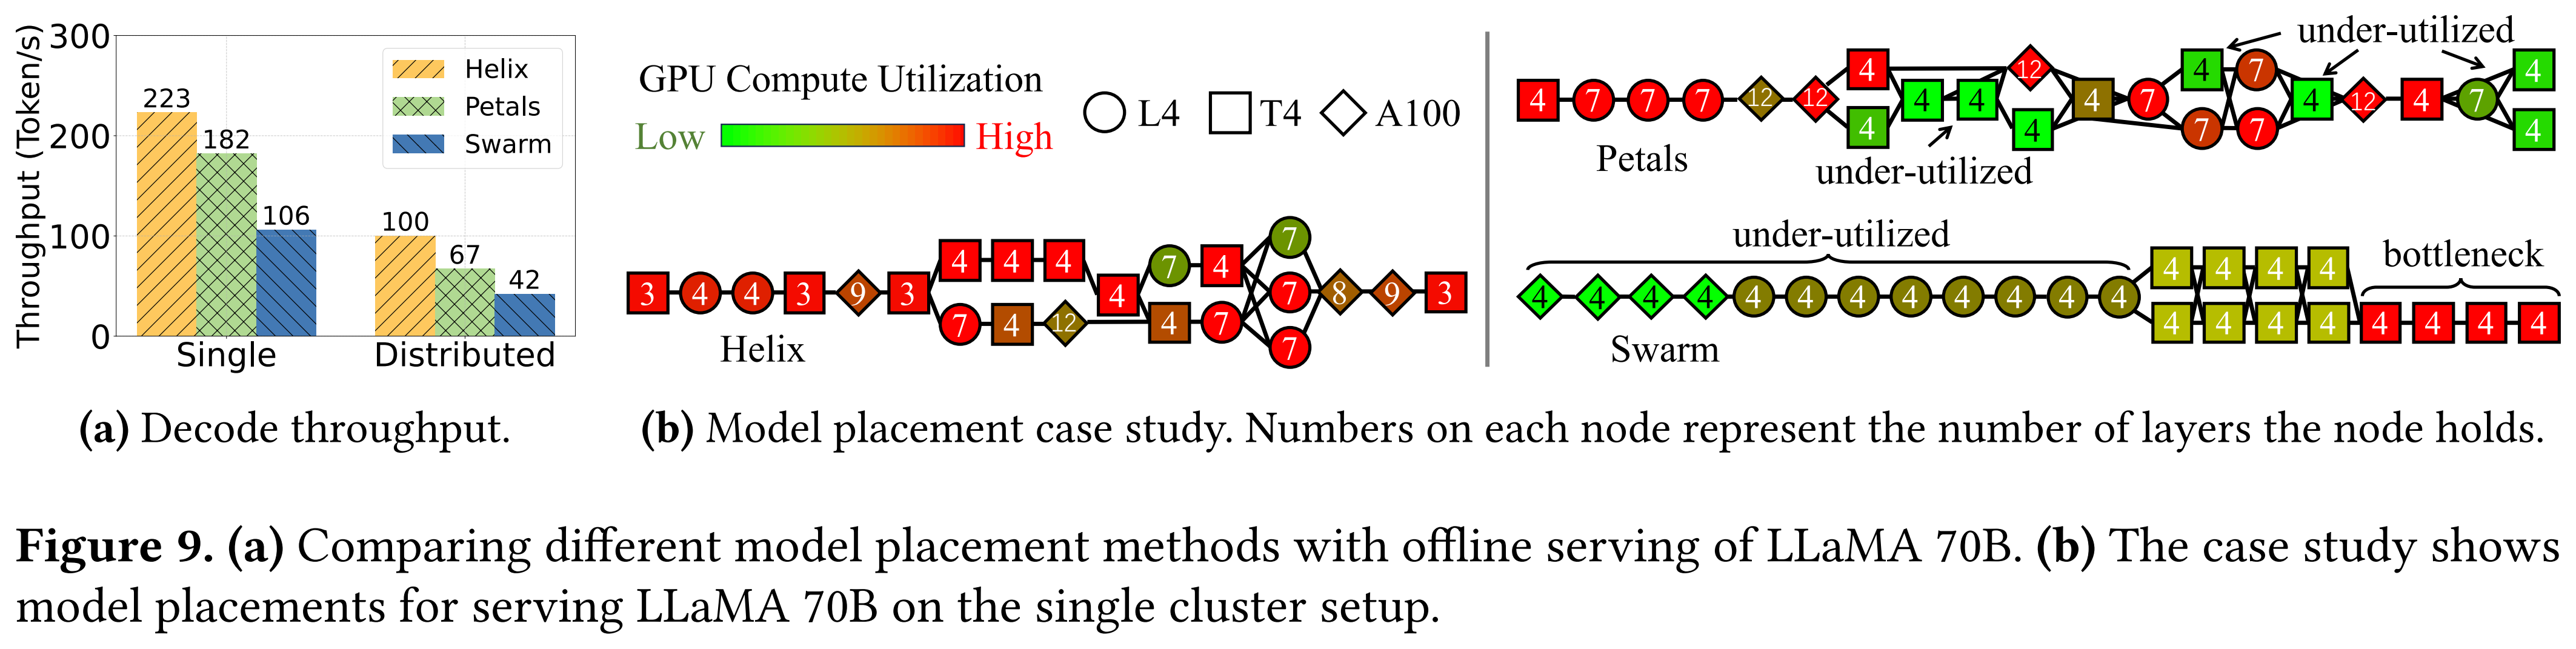
\includegraphics[width=\linewidth]{Helix/Helix_Figure_09_Model_Placement_Comparison.png}
\end{column}
\begin{column}{.49\textwidth}
{\footnotesize\textbf{Scheduling ablation.} Helix placement fixed.\par}
{\footnotesize vs.\ Swarm / random\par}
{\footnotesize Single: $+30\%$ / $+29\%$\quad Geo: $+22\%$ / $+15\%$\par}
\vspace{.02cm}
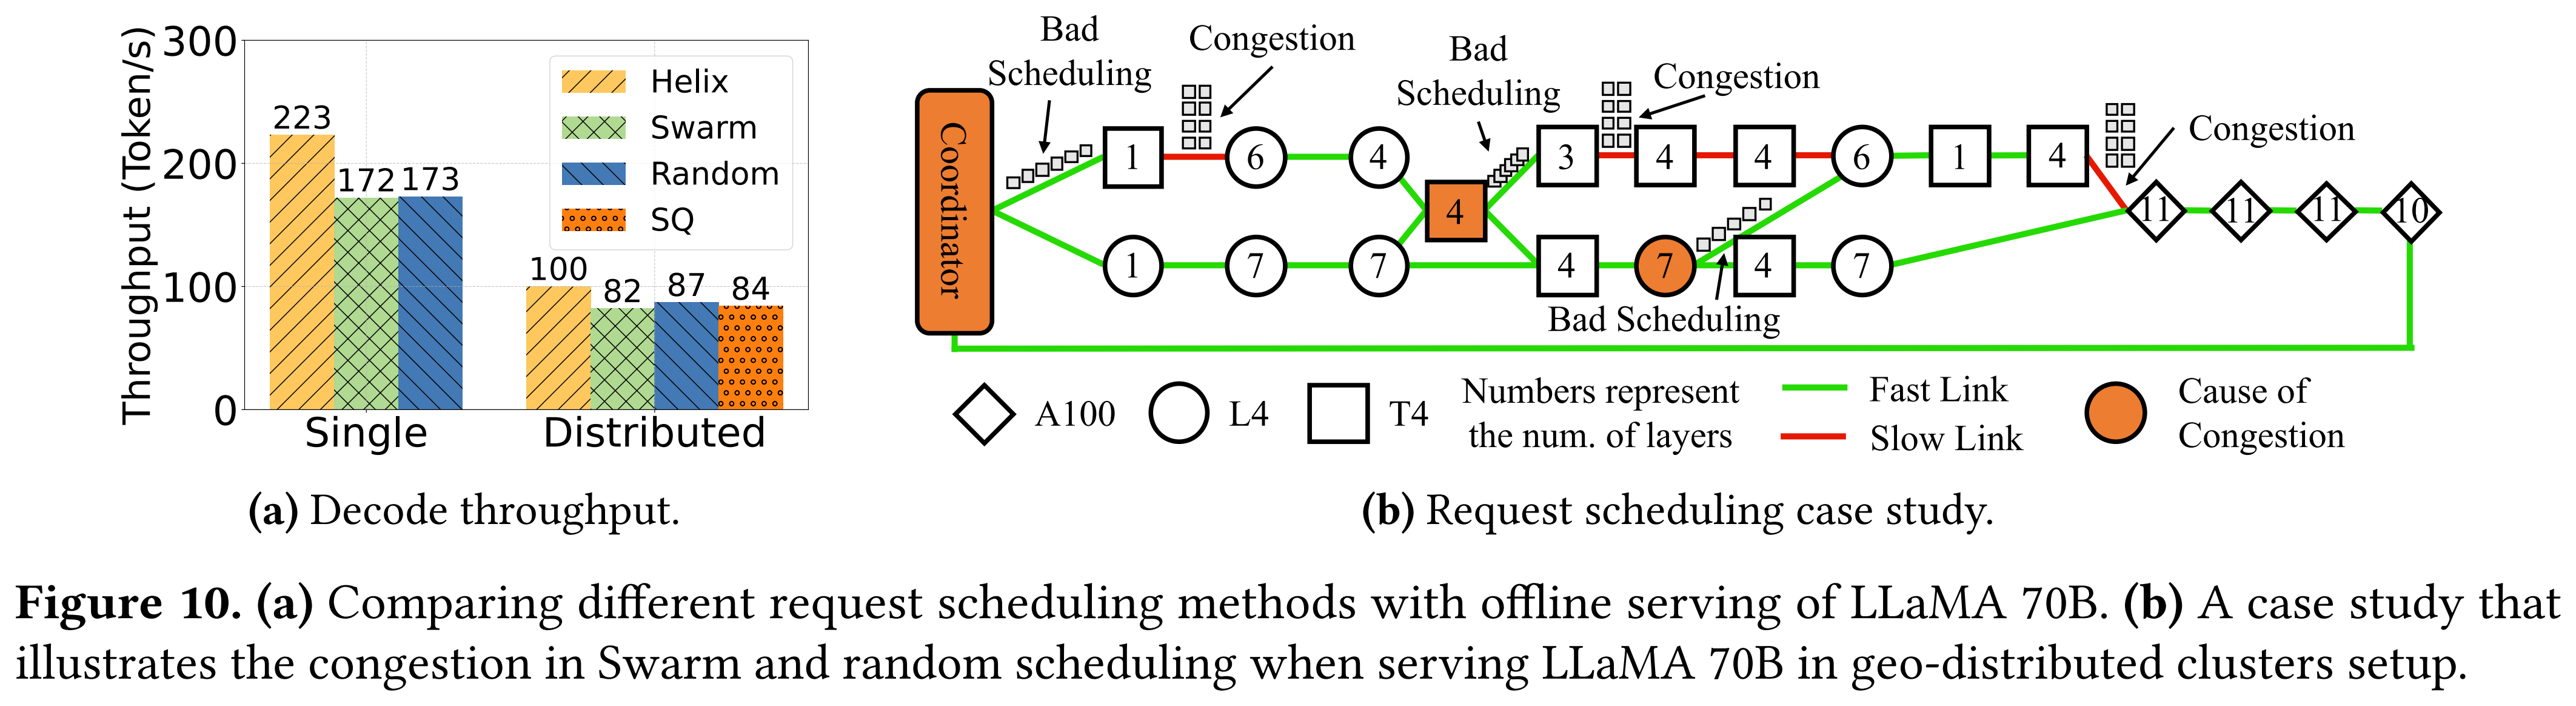
\includegraphics[width=\linewidth]{Helix/Helix_Figure_10_Request_Scheduling_Comparison.png}
\end{column}\end{columns}
\vspace{.12cm}\takeaway{Placement builds the resource graph. Scheduling is what actually uses that capacity.}
\src{Helix Sec.~6.6--6.7, Figs.~9--10. Geo-distributed bars are simulator results.}

\end{frame}

\begin{frame}[t]{Tessera: Why Is Phase-Level Disaggregation Too Coarse?}
{\footnotesize Tessera finds that the best GPU changes from kernel to kernel, so it places execution at GPU-kernel granularity.\par}
\vspace{.04cm}
\begin{columns}[T,onlytextwidth]
\begin{column}{.60\textwidth}
\mainfig{Tessera/Tessera_Figure_03_Kernel_Duration_Ratios.png}{5.15cm}
\end{column}
\begin{column}{.38\textwidth}
\vspace{.15cm}
{\footnotesize\textbf{GPT-oss 20B, A100 vs.\ L40s.}}
\vspace{.12cm}
{\footnotesize About \textbf{45\% of prefill} kernels and \textbf{57\% of decode} kernels are faster on L40s.}
\vspace{.12cm}
{\footnotesize Attention and FFN blocks are mixed too: a block name does not pick the GPU.}
\vspace{.12cm}
{\footnotesize Points below the dashed line prefer L40s. The 45\%/57\% figures count kernels, not execution time.}
\end{column}\end{columns}
\vspace{.10cm}\takeaway{A phase label is not a hardware preference.}
\src{Tessera Sec.~II-C, Fig.~3. X-axis: kernel duration on A100. Y-axis: L40s/A100 time.}
\end{frame}

\begin{frame}[t]{Tessera: How Does It Work?}

\begin{columns}[T,onlytextwidth]
\begin{column}{.46\textwidth}
\mainfig{Tessera/Tessera_Figure_04_System_Overview.png}{4.85cm}
\end{column}
\begin{column}{.52\textwidth}
\begin{enumerate}\footnotesize\setlength{\itemsep}{.08cm}
\item \textbf{Analyzer:} memory ranges and RAW dependencies. If B reads what A wrote, B waits for that data.
\item \textbf{Profiling:} each kernel's latency on each GPU type.
\item \textbf{Planner:} build DDGs and solve offline policies.
\item \textbf{Runtime:} workers run assigned kernels and transfers. The monitor selects a stored policy.
\end{enumerate}
\vspace{.10cm}
{\footnotesize\textbf{Throughput policy:} balance compute and communication when requests can overlap.}
\vspace{.08cm}
{\footnotesize\textbf{Latency policy:} at low load, shorten one request's compute plus the transfers that cannot be hidden.}
\end{column}\end{columns}
\vspace{.12cm}\takeaway{Analysis and MILP stay offline. Runtime only executes or switches stored policies.}
\src{Tessera Sec.~III, Fig.~4. RAW = Read After Write. The latency objective sums kernel and cut-edge costs.}

\end{frame}

\begin{frame}[t]{Q1: Does Kernel-Level Disaggregation Outperform Phase/Block-Level Methods?}

{\footnotesize\textbf{Question:} Does scheduling at kernel granularity raise end-to-end throughput, or only individual kernel speed?\par}
\vspace{.04cm}
\mainfig{Tessera/Tessera_Figure_06_Offline_Throughput.png}{3.15cm}
\vspace{.04cm}
{\footnotesize Five offline workloads, three GPU pairs. PD = prefill/decode. AF = attention/FFN.}
\begin{itemize}\footnotesize\setlength{\itemsep}{.08cm}
\item Vs.\ PD: $1.5\times$ average, up to $2.3\times$ throughput.
\item Vs.\ AF: $1.35\times$ average, up to $1.7\times$ throughput.
\end{itemize}
\vspace{.08cm}\takeaway{Kernel-level scheduling turns the motivation into end-to-end throughput gains.}
\src{Tessera Sec.~V-A--B, Fig.~6. Tokens/s; SD axis is images/min. Red X: baseline inapplicable.}

\end{frame}

\begin{frame}[t]{Q2: Can Tessera Sustain More Requests under the Same Latency SLO?}
{\footnotesize\textbf{Question:} Under arrivals and a latency cap, can Tessera carry a higher request rate?\par}
\vspace{.04cm}
\begin{columns}[T,onlytextwidth]
\begin{column}{.62\textwidth}
\mainfig{Tessera/Tessera_Figure_07_Online_Latency.png}{4.55cm}
\end{column}
\begin{column}{.36\textwidth}
{\footnotesize GPT-oss 20B, Poisson arrivals, three GPU pairs.}
\vspace{.12cm}
{\footnotesize\textbf{Low load:} normalized latency about $1.3\times$ / $1.2\times$ lower than PD / AF.}
\vspace{.12cm}
{\footnotesize\textbf{Same 50\,ms/token SLO:} up to about $1.3\times$ the request rate of the best baseline.}
\vspace{.12cm}
{\footnotesize Offline throughput and this SLO capacity are different regimes.}
\end{column}\end{columns}
\vspace{.10cm}\takeaway{The gain is not only saturated throughput. Stored policies also help online.}
\src{Tessera Sec.~V-B, Fig.~7. Normalized latency = end-to-end time / output tokens.}
\end{frame}

\begin{frame}[t]{Q3: Does Communication Overhead Cancel the Benefit of Kernel Splitting?}

{\footnotesize\textbf{Question:} Kernel splits add cross-GPU transfers. Can pipelining hide enough of that cost?\par}
\vspace{.04cm}
\mainfig{Tessera/Tessera_Figure_09_Pipeline_Effectiveness.png}{3.35cm}
\vspace{.04cm}
{\footnotesize\textbf{GPT-oss 20B, offline.} No pipeline 1443; pipeline 2123; pipeline + priority \textbf{2641 tokens/s}.}
\begin{itemize}\footnotesize\setlength{\itemsep}{.08cm}
\item Zero-communication reference: 2734 tokens/s. $2641/2734 \approx 96.6\%$.
\item Later requests use a lower CUDA stream priority, so their transfers do not all line up.
\end{itemize}
\vspace{.08cm}\takeaway{Placement alone is not enough. Overlap is a necessary runtime mechanism.}
\src{Tessera Sec.~III-C, V-D, Fig.~9. The reference assumes zero communication cost. GPU pair not named here.}

\end{frame}

\begin{frame}[t]{What Do Helix and Tessera Teach Us about Heterogeneous Serving?}

\small\renewcommand{\arraystretch}{1.20}
\begin{tabularx}{\textwidth}{@{}p{2.0cm}>{\raggedright\arraybackslash}p{3.2cm}>{\raggedright\arraybackslash}X@{}}\toprule
System & Optimization unit & Main question\\\midrule
ThunderServe & Prefill / decode phase & Which GPU group should serve each phase?\\
Helix & Layers + request pipeline & Where should layers go, and how should requests flow?\\
Hetis & Attention heads & How should attention work and KV state be distributed?\\
Tessera & GPU kernels & Which GPU should execute each kernel?\\\bottomrule
\end{tabularx}
\vspace{.18cm}
\textbf{Conclusion:} These systems optimize heterogeneity along different dimensions.\par\vspace{.12cm}
Finer granularity can expose hardware opportunities, but adds dependency tracking, communication, planning, and runtime coordination.\par
\vspace{.18cm}\takeaway{How fine should optimization become before communication and coordination costs outweigh the benefit?}
\src{Our project-level synthesis and open question, not a cross-paper performance ranking.}

\end{frame}

\appendix
\backuptrue
\begin{frame}[t]{Max-Flow Graph Abstraction}
  \smalllabel{Helix / Formulation}\par
  \vspace{.02cm}
  \begin{columns}[c,onlytextwidth]
    \begin{column}{.46\textwidth}
      {\footnotesize\begin{itemize}\setlength{\itemsep}{.08cm}
        \item Each compute node becomes \(c^{\mathrm{in}}\rightarrow c^{\mathrm{out}}\).
        \item The coordinator becomes the source and the sink.
        \item An edge capacity is how many tokens may cross it per second.
        \item Max flow from source to sink is the serving throughput of this placement.
      \end{itemize}}
      \vspace{.08cm}\takeaway{The graph is an accounting device for one fixed placement.}
    \end{column}
    \begin{column}{.52\textwidth}
      \figureplaceholder{Helix/Helix_Figure_02_Max_Flow_Graph_Abstraction.png}{5.15cm}{Figure 2}
      {\centering\hint{Fig.~2. Capacities are tokens/s.}\par}
    \end{column}
  \end{columns}
  \src{Sec.~4.3, Fig.~2. PDF p.~4.}
\end{frame}
\begin{frame}[t]{Modeling Compute Capacity}
  \smalllabel{Helix / Formulation}\par
  \vspace{.04cm}
  \begin{columns}[T,onlytextwidth]
    \begin{column}{.49\textwidth}
      \stepcard{NODE EDGE}{\(c^{\mathrm{in}}\rightarrow c^{\mathrm{out}}\)}{Capacity is the minimum of profiled compute throughput and the node's network throughput.}
      \vspace{.04cm}
      \stepcard{PROFILING}{Once per node}{Helix measures throughput rather than using the datasheet TFLOP/s from Table 3.}
    \end{column}
    \begin{column}{.49\textwidth}
      \stepcard{LAYER COUNT}{\(T_j\) tokens/s}{\(T_j\) is the profiled rate when that node holds \(j\) layers. It becomes the MILP compute limit.}
      \vspace{.04cm}
      \stepcard{NOT A GPU}{Source and sink}{The coordinator injects tokens and collects tokens. It is not given a compute edge.}
    \end{column}
  \end{columns}
  \vspace{.04cm}\takeaway{Compute capacity is a profiled token rate, and it already takes the node's network limit into account.}
  \src{Sec.~4.3. \(T_j\) is defined with Constraint~3 in Sec.~4.4.}
\end{frame}
\begin{frame}[t]{Modeling Network Capacity}
  \smalllabel{Helix / Formulation}\par
  \vspace{.08cm}
  {\footnotesize A link is valid only in one of three cases:}\par
  \vspace{.08cm}
  \begin{enumerate}\footnotesize
    \setlength{\itemsep}{.10cm}
    \item Coordinator \(\rightarrow\) a node that holds the first layer. Payload is a token (Fig.~2 uses 4 bytes).
    \item A node that holds the last layer \(\rightarrow\) coordinator. Payload is again a token.
    \item Node \(i\rightarrow\) node \(j\) when \(j\) holds the layers needed immediately after \(i\). Payload is an activation (Fig.~2 uses 16 KB).
  \end{enumerate}
  \vspace{.08cm}
  \[
    \text{capacity (tokens/s)}=\frac{\text{profiled average bandwidth}}{\text{bytes per token or activation}}.
  \]
  {\footnotesize The formula is the paper's rule. The byte sizes above are the Fig.~2 annotations, not universal constants.}\par
  \vspace{.12cm}\takeaway{Activations cost far more tokens of budget than the final output token, so wide-area links saturate first.}
  \src{Sec.~4.3. Bandwidth is a one-time average, not a runtime measurement.}
\end{frame}
\begin{frame}[t]{Why Max Flow Represents Serving Throughput}
  \smalllabel{Helix / Formulation}\par
  \vspace{.10cm}
  \begin{itemize}\footnotesize
    \setlength{\itemsep}{.08cm}
    \item One unit of flow is one token that can pass a node or a link in one second.
    \item Conservation forces tokens into \(c^{\mathrm{in}}\) to leave through \(c^{\mathrm{out}}\).
    \item Helix computes the source--sink max flow with preflow-push. That value is the placement's max serving throughput.
    \item The model is a steady token rate. It does not output prompt latency, decode latency, or a percentile.
    \item A later early-stop bound is the sum of node compute rates, divided by the number of layers.
  \end{itemize}
  \vspace{.08cm}\takeaway{Max flow answers ``how many tokens/s can this placement carry?'' It is not a latency model.}
  \src{Sec.~4.3 and the early-stop remark in Sec.~4.5.}
\end{frame}
\begin{frame}[t]{MILP Variables and Objective}
  \smalllabel{Helix / MILP}\par
  \vspace{.06cm}
  {\centering\footnotesize
  \begin{tabular}{lll}\toprule
    Symbol & Role & Meaning\\\midrule
    \(s_i\) & integer & first layer on node \(i\)\\
    \(b_{ij}\) & binary & node \(i\) holds exactly \(j\) layers\\
    \(f_{i,j}\) & real & flow from \(i\) to \(j\), in tokens/s\\
    \(d_{i,j}\) & binary & whether link \((i,j)\) is valid\\
    \(\mathit{cond}\) & binary & auxiliaries that linearize overlap\\\bottomrule
  \end{tabular}\par}
  \vspace{.08cm}
  {\footnotesize \(e_i=s_i+\sum_j j\,b_{ij}\). Node \(i\) holds the half-open range \([s_i,e_i)\). \(k\) is the most layers that fit on that GPU.}\par
  \vspace{.06cm}
  \[
    \max \sum_i f_{\mathrm{source},i}
  \]
  \vspace{.08cm}\takeaway{The objective maximizes coordinator outflow. Table 5 groups the variable counts as linear in \(|C|\) or \(|E|\).}
  \src{Sec.~4.4, Tables 5--6. Notation here is compacted from the paper.}
\end{frame}
\begin{frame}[t]{Placement and Memory Constraints}
  \smalllabel{Helix / MILP}\par
  \vspace{.10cm}
  \[
    \sum_{j=1}^{k} b_{ij}=1,
    \qquad 0\le s_i<L,
    \qquad e_i\le L.
  \]
  \begin{itemize}\footnotesize
    \setlength{\itemsep}{.07cm}
    \item Exactly one layer-count is chosen. The range must lie inside the model's \(L\) layers.
    \item Memory enters as \(k\), the maximum number of layers the GPU can hold. Table 6 has no KV-byte variable.
    \item If \(s_j<e_i<e_j\), traffic from \(i\) runs only layers \([e_i,e_j)\) on \(j\). The paper calls this partial inference.
    \item The solver may be run with partial inference disabled. Then a link is valid only when \(e_i=s_j\).
  \end{itemize}
  \vspace{.12cm}\takeaway{GPU memory limits how many layers are placed. KV capacity is enforced later, at schedule time.}
  \src{Sec.~4.4, Constraint~1, and the partial-inference remark.}
\end{frame}
\begin{frame}[t]{Flow and Compute Constraints}
  \smalllabel{Helix / MILP}\par
  \vspace{.12cm}
  {\footnotesize\textbf{Constraint 2: conservation at node \(i\).}}\par
  \[
    \sum_u f_{u,i}=\sum_v f_{i,v}.
  \]
  {\footnotesize\textbf{Constraint 3: profiled inference throughput.}}\par
  \[
    \sum_u f_{u,i}\le \sum_{j=1}^{k} b_{ij}\,T_j.
  \]
  \begin{itemize}\footnotesize
    \setlength{\itemsep}{.04cm}
    \item \(T_j\) is a profiled constant: tokens per second when this node holds \(j\) layers.
    \item The binaries \(b_{ij}\) pick exactly one of those profiled rates.
    \item Flow is still also limited by the network edges on the next slide.
  \end{itemize}
  \vspace{.02cm}\takeaway{A node cannot be assigned more token flow than the profiled rate for the layer count it actually holds.}
  \src{Sec.~4.4, Constraints 2--3. Sums skip node \(i\) itself, as stated in the paper.}
\end{frame}
\begin{frame}[t]{Connectivity and Network Constraints}
  \smalllabel{Helix / MILP}\par
  \vspace{.06cm}
  {\footnotesize\textbf{Constraint 4, compacted.} A coordinator link into \(i\) exists only if \(i\) holds the first layer:}\par
  \[
    s_i\le L\,(1-d_{\mathrm{source},i}).
    \qquad
    L\,d_{i,\mathrm{sink}}\le e_i.
  \]
  {\footnotesize Between compute nodes, \(d_{ij}=1\) only if \(s_j\le e_i<e_j\). Two auxiliary binaries linearize that test, and \(d_{ij}\le 0.5\,\mathit{cond}^{1}+0.5\,\mathit{cond}^{2}\).}\par
  \vspace{.06cm}
  {\footnotesize\textbf{Constraint 5: transmission throughput.}}\par
  \[
    f_{ij}\le d_{ij}\,S_{ij}.
  \]
  {\footnotesize \(S_{ij}\) is the profiled token rate of that link, from Sec.~4.3. Invalid links carry zero flow.}\par
  \vspace{.10cm}\takeaway{Routing variables cannot use a hop that the layer ranges do not justify.}
  \src{Sec.~4.4, Constraints 4--5. The two-auxiliary form is the paper's linearization.}
\end{frame}
\begin{frame}[t]{Converting Max-Flow Weights into Scheduling}
  \smalllabel{Helix / Runtime}\par
  \vspace{.02cm}
  \begin{columns}[T,onlytextwidth]
    \begin{column}{.49\textwidth}
      \stepcard{IWRR}{Interleaved weighted round-robin}{Each vertex has a scheduler. A neighbor's weight is the max-flow value on that outgoing edge.}
      \vspace{.01cm}
      \stepcard{WHY INTERLEAVE}{Avoid bursts}{Frequency follows the weight, but choices are interleaved so one heavy edge is not drained in a burst.}
    \end{column}
    \begin{column}{.49\textwidth}
      \stepcard{THE WALK}{Coordinator, then each node}{Pick stage 1 from the coordinator. Pick stage 2 from that node's scheduler. Stop when the path is complete.}
      \vspace{.01cm}
      \stepcard{MASK}{Before the walk}{Nodes over the KV high-water mark are removed from the candidate list. This avoids scheduling onto a full KV cache.}
    \end{column}
  \end{columns}
  \takeaway{The MILP decides the rates. IWRR is the online rule that realizes those rates.}
  \src{Sec.~5.1. IWRR follows Tabatabaee et al.\ as cited by the paper.}
\end{frame}
\begin{frame}[t]{Pipeline Scheduling Example}
  \smalllabel{Helix / Runtime}\par
  \vspace{.02cm}
  \begin{columns}[c,onlytextwidth]
    \begin{column}{.46\textwidth}
      {\footnotesize\begin{itemize}\setlength{\itemsep}{.07cm}
        \item Vertices are compute nodes. An edge exists only if the MILP placement made it valid.
        \item The number on an edge is flow in the max-flow solution, not link capacity.
        \item The figure's two example pipelines are \(1\rightarrow 5\rightarrow 9\) and \(2\rightarrow 6\rightarrow 8\).
        \item Those paths can share the cluster. They are not two frozen replicas.
      \end{itemize}}
      \vspace{.12cm}\takeaway{Read the integers as scheduled token rates, then read the paths as two requests.}
    \end{column}
    \begin{column}{.52\textwidth}
      \figureplaceholder{Helix/Helix_Figure_04_Per_Request_Pipeline_Scheduling.png}{4.85cm}{Figure 4}
    \end{column}
  \end{columns}
  \src{Sec.~5.1, Fig.~4. PDF p.~8.}
\end{frame}
\begin{frame}[t]{High GPU-Heterogeneity Results}
  \smalllabel{Helix / Results}\par
  \vspace{.02cm}
  \begin{columns}[c,onlytextwidth]
    \begin{column}{.48\textwidth}
      {\footnotesize\begin{itemize}\setlength{\itemsep}{.09cm}
        \item Simulator, LLaMA 70B, 42 nodes, 7 types. V100, T4, and \(2\times\)T4 cannot form a pipeline alone.
        \item SP drops those machines. SP+ adds a mixed pipeline that uses them.
        \item Vs.\ Swarm / SP / SP+, offline throughput is \(1.37\times\), \(2.91\times\), \(2.24\times\).
        \item Online: \(1.48\times\), \(3.29\times\), \(2.54\times\). Prompt latency changes by \(-17\%\), \(-1\%\), \(-7\%\).
        \item Helix's decode latency is slightly higher: baselines leave slow GPUs idle.
      \end{itemize}}
      \vspace{.10cm}\takeaway{The abstract's \(3.3\times\) is the \(3.29\times\) online gain versus SP, rounded.}
    \end{column}
    \begin{column}{.50\textwidth}
      \figureplaceholder{Helix/Helix_Figure_08_High_GPU_Heterogeneity_Results.png}{4.70cm}{Figure 8}
    \end{column}
  \end{columns}
  \src{Sec.~6.5, Fig.~8. PDF p.~10. Not a prototype measurement.}
\end{frame}
\begin{frame}[t]{MILP Optimization Ablation}
  \smalllabel{Helix / Ablation}\par
  \vspace{.02cm}
  \begin{columns}[c,onlytextwidth]
    \begin{column}{.46\textwidth}
      {\footnotesize\begin{itemize}\setlength{\itemsep}{.09cm}
        \item Offline LLaMA 70B. 24-node is the geo setup; 42-node is the high-heterogeneity setup.
        \item Degree-12 pruning drops 50\% and 72\% of the links, and 36\% and 46\% of the problem size.
        \item With pruning, decode throughput is 16\% and 2\% higher. The paper attributes this to an easier search under a time limit.
        \item Warm start finds the same placement, in 43\% and 8\% less wall time.
      \end{itemize}}
    \end{column}
    \begin{column}{.52\textwidth}
      \figureplaceholder{Helix/Helix_Figure_11_MILP_Optimization_Ablation.png}{3.15cm}{Figure 11}
      {\centering\scriptsize
      \begin{tabular}{lcc}\toprule
        & With pruning & Without\\\midrule
        24-node & 876 var, 1122 cstr & 1376 var, 1848 cstr\\
        42-node & 2144 var, 2772 cstr & 4004 var, 5502 cstr\\\bottomrule
      \end{tabular}\par}
    \end{column}
  \end{columns}
  \vspace{.10cm}\takeaway{Pruning changes the search problem. It is not a proof that the deleted links were useless.}
  \src{Sec.~6.8, Fig.~11, Table 8. PDF p.~12. Speedups vary by instance, as the paper notes.}
\end{frame}
\begin{frame}[t]{Solver Time and Solution Quality}
  \smalllabel{Helix / Ablation}\par
  \vspace{.02cm}
  \begin{columns}[c,onlytextwidth]
    \begin{column}{.48\textwidth}
      {\footnotesize\begin{itemize}\setlength{\itemsep}{.07cm}
        \item Instance: LLaMA 30B on 4 L4s and 6 T4s. This is smaller than the 24- and 42-node runs.
        \item The best feasible placement reaches the optimum in under 5 minutes.
        \item Certifying that optimum takes more than an hour of branch-and-bound.
        \item The red dotted line is that cluster's optimal throughput. The upper bound tightens as cuts are added.
      \end{itemize}}
      \vspace{.12cm}\takeaway{Early stop is reasonable here. Fig.~12 does not certify the 42-node plan.}
    \end{column}
    \begin{column}{.50\textwidth}
      \figureplaceholder{Helix/Helix_Figure_12_MILP_Solution_Quality.png}{4.85cm}{Figure 12}
    \end{column}
  \end{columns}
  \src{Sec.~6.9, Fig.~12. PDF p.~13.}
\end{frame}
\begin{frame}[t]{PTX Instrumentation and Address Ranges}
  \smalllabel{Tessera / Analyzer}\par
  \vspace{.08cm}
  \begin{enumerate}\footnotesize
    \setlength{\itemsep}{.07cm}
    \item Add an instrumentation buffer to the kernel parameters and load it with \texttt{ld.param}.
    \item Around each \texttt{ld.global} / \texttt{st.global}, emit \texttt{atom.global.min} and \texttt{atom.global.max} so threads agree on one range.
    \item After the launch, align each instruction's \([\min,\max]\) interval with buffer base addresses. The opcode says read or write.
    \item Recompile the patched PTX with \texttt{ptxas}. The probe engine is built on NEUTRINO.
  \end{enumerate}
  \vspace{.06cm}
  {\footnotesize If a kernel touches a global that is not a launch argument, the base address is unknown. Tessera then refuses to disaggregate that kernel. The paper cites a study that this pattern is absent in PyTorch and vLLM, and present in one Rodinia kernel.}\par
  \vspace{.05cm}\takeaway{The analyzer records touched address ranges. It does not reconstruct a kernel's arithmetic.}
  \src{Sec.~III-A and Sec.~IV. Listing 1 is the paper's instrumentation sketch.}
\end{frame}
\begin{frame}[t]{Extracting RAW Dependencies}
  \smalllabel{Tessera / Analyzer}\par
  \vspace{.10cm}
  \begin{itemize}\footnotesize
    \setlength{\itemsep}{.08cm}
    \item Execution order is preserved, so only Read-After-Write edges can change the result. WAR and WAW are not the edges Tessera schedules.
    \item A registry stores the last writer of each buffer. A later reader adds an edge from that writer, annotated with the measured byte size.
    \item Asynchronous copies are nodes too. Their source, destination, and size come from the API.
    \item One CUDA graph gets one dependency graph. Dynamic shapes become several graphs, not one graph with a runtime branch.
    \item Frameworks without CUDA Graph can record a trace and replay it under stream capture. That tool is preprocessing, not the online scheduler.
  \end{itemize}
  \vspace{.12cm}\takeaway{The graph is a static RAW graph per captured execution, plus the byte size of each edge.}
  \src{Sec.~III-A. ``DDG'' is the paper's term for this graph.}
\end{frame}
\begin{frame}[t]{Cross-Iteration Dependencies and KV State}
  \smalllabel{Tessera / Analyzer}\par
  \vspace{.10cm}
  \begin{itemize}\footnotesize
    \setlength{\itemsep}{.08cm}
    \item The default graph is intra-iteration. KV cache is written in one iteration and read in a later one.
    \item The analyzer flags those buffers by profiling more than one iteration.
    \item At runtime each GPU keeps a replica. Only the delta is copied, asynchronously.
    \item Two NCCL communicators separate this background copy from the latency-critical cut-edge transfers. Dependency traffic gets the higher class.
    \item The paper says delta replication is under 0.1\% of latency, citing prior prefill/decode work rather than a new Tessera measurement.
  \end{itemize}
  \vspace{.12cm}\takeaway{KV state is replicated and updated in the background. It is not a cut edge on the per-iteration critical path.}
  \src{Sec.~III-A and Sec.~IV. The 0.1\% figure is attributed to prior work [9], [10].}
\end{frame}
\begin{frame}[t]{Offline Throughput-Oriented MILP}
  \smalllabel{Tessera / Planner}\par
  \vspace{.08cm}
  \[
    \sum_{g\in G} x_{k,g}=1,
    \qquad
    T_g=\sum_{k\in K} t_{k,g}\,x_{k,g},
    \qquad
    W_g=\max(T_g,M_g),
    \qquad
    \min \max_{g\in G} W_g.
  \]
  \begin{itemize}\footnotesize
    \setlength{\itemsep}{.10cm}
    \item \(T_g\) is compute time on GPU \(g\). \(M_g\), on the next slide, is communication time into \(g\).
    \item \(W_g\) is the slower of the two. Steady-state throughput is then one request per \(\max_g W_g\).
    \item This is the offline objective. It is the wrong objective when too few requests are in flight to hide transfers.
    \item Gurobi solves it offline. A reported case, GPT-oss 20B on A100+L40s, has about 500 kernels and finishes one graph in about 20 ms.
  \end{itemize}
  \vspace{.10cm}\takeaway{The MILP balances GPUs by minimizing the slowest stage. It does not maximize a sum of kernel speeds.}
  \src{Sec.~III-B. The 20 ms figure is for \(|G|=2\), \(|K|\approx 500\); all patterns take about 5 s.}
\end{frame}
\begin{frame}[t]{Communication and Load-Balancing Constraints}
  \smalllabel{Tessera / Planner}\par
  \vspace{.06cm}
  \[
    c^{u,g}_{ij}=\ell_{u,g}+\frac{d_{ij}}{bw_{u,g}},
    \qquad
    M_g=\sum_{(i,j)\in E}\sum_{u\in G\setminus\{g\}} c^{u,g}_{ij}\,y^{u,g}_{ij}.
  \]
  \begin{itemize}\footnotesize
    \setlength{\itemsep}{.10cm}
    \item \(y^{u,g}_{ij}=x_{i,u}x_{j,g}\) is 1 when the producer is on \(u\) and the consumer is on \(g\). The product is linearized with the standard Boolean replacement.
    \item Load balance is not a separate variance constraint. Minimizing \(\max_g W_g\) already penalizes the busiest GPU.
    \item Per-GPU memory capacity is absent. At initialization every GPU receives a full copy of the weights.
    \item Offline, once the policy is fixed, unused weight buffers can be reclaimed. The paper does not report that reclamation in the evaluation tables.
  \end{itemize}
  \vspace{.10cm}\takeaway{Communication is bytes over profiled bandwidth, plus a base latency. Memory is a runtime caveat, not a constraint.}
  \src{Sec.~III-B and Sec.~IV. Linearization cites Nemhauser and Wolsey.}
\end{frame}
\begin{frame}[t]{Online Latency-Oriented Scheduling}
  \smalllabel{Tessera / Planner}\par
  \vspace{.08cm}
  {\footnotesize Under low load the pipeline cannot hide transfers. The objective adds kernel time and cut-edge transfer time:}\par
  \[
    \min \sum_{k,g} t_{k,g}x_{k,g}
    +\sum_{(i,j)}\sum_{u}\sum_{g\neq u} c^{u,g}_{ij}\,y^{u,g}_{ij}.
  \]
  \begin{itemize}\footnotesize
    \setlength{\itemsep}{.09cm}
    \item There is no \(\max(T,M)\) here. Overlap is not assumed.
    \item The same Gurobi solve is offline. Workers only look up the stored policy.
    \item If communication is expensive, this objective keeps dependent kernels on the same GPU. Fig.~11 shows that behavior at 25 Gb/s.
  \end{itemize}
  \vspace{.10cm}\takeaway{Latency mode shortens one request's critical path. It is not the throughput MILP with a different label.}
  \src{Sec.~III-B. The sum is the paper's low-load decomposition, compacted for the slide.}
\end{frame}
\begin{frame}[t]{GPU Worker Execution}
  \smalllabel{Tessera / Execution}\par
  \vspace{.02cm}
  \begin{columns}[c,onlytextwidth]
    \begin{column}{.48\textwidth}
      {\footnotesize\begin{itemize}\setlength{\itemsep}{.09cm}
        \item Fig.~5 is GPU B from the six-kernel example. Compute and communication use different streams.
        \item \(R_{ij}\) receives kernel \(i\)'s output for kernel \(j\). \(S_{ij}\) sends it. CUDA events order the two streams.
        \item Receives are posted before the consumer kernel. Sends are posted after the producer if the edge is cut.
        \item Sends and receives are GPU-side kernels via NCCL's GPUDirect Async (IBGDA), so the CPU is not on the critical path.
      \end{itemize}}
      \vspace{.10cm}\takeaway{A worker runs its own kernels and the cut-edge messages. It does not run the whole model.}
    \end{column}
    \begin{column}{.50\textwidth}
      \figureplaceholder{Tessera/Tessera_Figure_05_GPU_Worker_Execution.png}{4.15cm}{Figure 5}
    \end{column}
  \end{columns}
  \src{Sec.~III-C, Fig.~5. PDF p.~6.}
\end{frame}
\begin{frame}[t]{Online Monitor Signals}
  \smalllabel{Tessera / Runtime}\par
  \vspace{.04cm}
  \begin{itemize}\footnotesize
    \setlength{\itemsep}{.01cm}
    \item The monitor records per-request latency, communication time, and per-kernel-group latency.
    \item A kernel group is the run of kernels between two consecutive communication operations. Individual kernels are not timed online.
    \item \(\bar L_{\mathrm{req}}\) is average end-to-end request latency. \(\bar L_{\mathrm{exec}}\) sums compute and communication and excludes queueing.
    \item The pressure signal is the ratio \(\bar L_{\mathrm{req}}/\bar L_{\mathrm{exec}}\).
    \item A low ratio means little queueing, so the latency policy is preferred. A high ratio means queueing dominates, so the throughput policy is preferred.
  \end{itemize}
  \vspace{.02cm}\takeaway{The switch looks at queueing pressure, not at a hand-named GPU counter.}
  \src{Sec.~III-D. Kernel group is the paper's definition.}
\end{frame}
\begin{frame}[t]{Policy Switching and Sensitivity Parameters}
  \smalllabel{Tessera / Runtime}\par
  \vspace{.02cm}
  \begin{columns}[T,onlytextwidth]
    \begin{column}{.49\textwidth}
      \stepcard{WINDOW \(W\)}{How often to decide}{The ratio is computed at window boundaries. The chosen defaults are \(W=300\) ms and \(\beta=1.5\).}
      \stepcard{THRESHOLD \(\beta\)}{When queueing wins}{Crossing \(\beta\) selects the throughput policy. Staying below it selects the latency policy.}
    \end{column}
    \begin{column}{.49\textwidth}
      \stepcard{SWITCH COST}{About 30 ms}{Workers synchronize on an iteration boundary. The 30 ms is the paper's reported stall, not a bound.}
      \stepcard{WHERE IT WAS TUNED}{One trace}{GPT-oss 20B, 360 s of the Azure Conversation trace. Fig.~10 is the sensitivity plot.}
    \end{column}
  \end{columns}
  \takeaway{\(W\) and \(\beta\) are the only two knobs the paper names. Aggressive and lazy settings both increase latency.}
  \src{Sec.~III-D and Sec.~V-D. Sensitivity measurements are in Fig.~10 of the paper.}
\end{frame}
\begin{frame}[t]{Network Bandwidth and MILP Analysis}
  \smalllabel{Tessera / Drill-down}\par
  \vspace{.02cm}
  \figureplaceholder{Tessera/Tessera_Figure_11_Network_Bandwidth_and_MILP.png}{2.05cm}{Figure 11}
  {\centering\hint{Fig.~11. (a) GPT-oss 20B, A100+L40s. (b) Gurobi time vs.\ kernels per graph.}\par}
  \vspace{.02cm}
  {\footnotesize\textbf{(a)} Throughput at 200 / 100 / 50 / 25 Gb/s: 2641 / 2610 / 2550 / 2490 tokens/s. The 25 Gb/s drop is under 6\%. Normalized latency: 1.00 / 1.03 / 1.08 / 1.15, still below the homogeneous A100 line at 1.18.}\par
  \vspace{.02cm}
  {\footnotesize\textbf{(b)} Text, 2 GPUs: 0.07 s at 200 kernels and 0.43 s at 1000 kernels. A DeepSeek-V3 671B forward graph of about 1500 kernels solves within 1 s. That is a solver stress test, not a serving result. Time grows with the number of GPU types; repeated layers are solved once.}\par
  \vspace{.08cm}\takeaway{At 25 Gb/s the offline pipeline still hides most of the extra delay. The latency policy moves work off the slow cut.}
  \src{Sec.~V-D, Fig.~11. PDF p.~10. Do not read panel (b) as an end-to-end DeepSeek result.}
\end{frame}
\begin{frame}[t]{Cost Efficiency of Heterogeneous Pairing}
  \smalllabel{Tessera / Results}\par
  \vspace{.06cm}
  {\footnotesize\textbf{Table III.} Perf/\$: mean throughput over the five workloads, divided by rental cost, then normalized to the left GPU alone. A pair pays for both GPUs.}\par
  \vspace{.05cm}
  {\centering\footnotesize
  \begin{tabular}{lccc}\toprule
    System & A100+L40s & H100+RTX Pro 6000 & B200+H100\\\midrule
    Homogeneous left & 1.00 & 1.00 & 1.00\\
    Homogeneous right & 1.18 & 2.01 & 0.78\\
    PD disaggregation & 0.87 & 1.00 & 0.70\\
    AF disaggregation & 1.02 & 1.07 & 0.74\\
    Tessera & 1.21 & 1.64 & 1.01\\\bottomrule
  \end{tabular}\par}
  \vspace{.06cm}
  \begin{itemize}\footnotesize
    \setlength{\itemsep}{.08cm}
    \item Vs.\ PD: \(1.5\times\) cost efficiency on average, up to \(1.6\times\). Vs.\ AF: \(1.4\times\) on average, up to \(1.5\times\).
    \item On H100+RTX Pro 6000, Tessera is \(1.64\times\) the Perf/\$ of H100 alone and \(2.3\times\) its throughput, above two H100s, at price \(2.9+1.2\) versus \(2\times 2.9\).
  \end{itemize}
  \vspace{.10cm}\takeaway{The pair can beat a single expensive GPU on Perf/\$. The prices are Table I's relative rentals, not a new quote.}
  \src{Sec.~V-B, Table III. The \(2.3\times\) sentence is the cost-efficiency paragraph, not the PD maximum.}
\end{frame}
\begin{frame}[t]{Generality Across Model Families}
  \smalllabel{Tessera / Results}\par
  \vspace{.06cm}
  {\centering\footnotesize
  \begin{tabularx}{\textwidth}{@{}>{\raggedright\arraybackslash}p{3.3cm}*{2}{>{\raggedright\arraybackslash}X}@{}}\toprule
    What was run & Models & What it does not show\\\midrule
    Offline pairs & Llama-3 8B, GPT-oss 20B, Qwen2.5-VL 7B, Mamba-Codestral 7B, SD 3.5 & PD or AF is inapplicable on some families\\
    Online SLO & GPT-oss 20B only & Latency for SSM, MLLM, or diffusion\\
    Cluster, offline & GPT-oss 20B and Qwen-3 235B & The single-pair Fig.~6 suite\\
    Solver stress test & DeepSeek-V3 671B, one forward graph & End-to-end serving\\\bottomrule
  \end{tabularx}\par}
  \vspace{.08cm}
  \begin{itemize}\footnotesize
    \setlength{\itemsep}{.09cm}
    \item AF needs an attention block, so Mamba and diffusion are out. PD needs a prefill/decode split, so diffusion is out.
    \item The motivation profiles say ``Mamba 7B''; the evaluated SSM is Mamba-Codestral 7B. Do not merge the two names.
  \end{itemize}
  \vspace{.12cm}\takeaway{``Four families'' means the offline pair study. Online evidence is one LLM.}
  \src{Sec.~II-B, Sec.~V-A--V-D. DeepSeek-V3 is the solver paragraph in Sec.~V-D.}
\end{frame}
\end{document}
